\chapter{Marco teórico}
\label{ch:marco}

\section{Descripción}

Toda tesis hace referencia a trabajos previos en el área y trabajos afines que
están directamente relacionados con lo planteado en el tesis.

Además, en el marco teórico debe aparecer la información absolutamente
necesaria para comprender la solución, y por eso es recomendable escribir
primero la solución (el siguiente capítulo), para ir anotando qué debe ser
explicado en el marco teórico.

\section{Generalidades}

Se recomienda revisar las guías de publicación de la \nt{IEEE} en
\url{http://www.ieee.org/publications_standards/publications/authors/authors_journals.html},
donde puede encontrar cómo hacer referencias bibliográficas
correctamente, cómo citar ecuaciones, cuadros y figuras, etc.  Además,
puede buscar en Google por la última versión del ``Biblatex Cheat
Sheet'' para el resumen de cómo construir correctamente cada
referencia.

\subsection{Redacción}

La \nt{redacción} en todo el documento debe seguir un estilo científico
objetivo. Esto implica que se redacta de modo impersonal, sin utilizar primeras
personas del singular o del plural, y se evita el uso de cualquier tipo de
calificativo, sustituyéndolos siempre por datos concretos, vinculados a
referencias bibliográficas o datos experimentales. Los comparativos también
deben concretarse a hechos y datos, y nunca dejarse ``en el aire''. Por la
naturaleza de la tesis, el tiempo verbal es usualmente presente, no perdiendo
nunca de vista que se está explicando ``cómo hacer algo'', en vez de ``qué se
hizo''.

Las \nt{frases} deben ser cortas, y debe evitarse que el lector tenga que saltar
constantemente entre partes de la tesis, lo que implica una exposición lineal
clara, donde lo que se necesita ya ha sido explicado antes. Deben evitarse
redundancias y por tanto cada concepto se exponen en un único lugar.

Todo aspecto circunstancial es irrelevante para la tesis, es decir, si se ha
desarrollado en el laboratorio $X$, o en el curso $Y$, con el profesor $Z$, o
en la empresa $W$, el nombre de funciones o clases en su código, etc., es
información irrelevante para reproducir el experimento, y por lo tanto sobra.
%
Esa información puede incluirse en uno de los anexos.


\subsubsection{Numeración del documento}

La primera página de la tesis es la correspondiente a la introducción,
así que ésta debe ser la página 1. Desde la introducción, hasta antes
de la bibliografía, las unidades son ``Capítulos''. La bibliografía y
anexos no se consideran capítulos, así que ya no continúan con la
misma numeración de los capítulos (la paginación sí continua). Los
índices, notación, glosario, etc.\ se numeran con números romanos en
versalitas ({\textsc{I}, \textsc{II}, \textsc{III}, \textsc{IV},
  \textsc{V}, \textsc{VI}}$\ldots$) y antes del índice (portada,
resúmenes, agradecimientos, hoja de evaluadores, etc.) las páginas no
llevan numeración.

Esta plantilla LaTeX ya se ocupa de todo lo anterior.

\subsection{Ecuaciones}

Para citar \nt{ecuaciones} se utilizan siempre paréntesis redondos, y
no es necesario emplear explícitamente la palabra ``ecuación''. Por
ejemplo ``Introduciendo en (4.2) los resultados de (3.3) y (3.7) se
obtiene ...''.  Se usa la palabra ``Ecuación'' solo si la frase inicia
con ello.  Por ejemplo ``La ecuación~\equ{eq:ej1} permite calcular la
corriente.''.

A diferencia de figura y cuadro, toda ecuación es parte del flujo de
texto y no un objeto flotante, así que \textbf{no} pueden emplearse de
la misma forma que las figuras o cuadros.  Esto es, cuando se requiere
introducir una ecuación, se pone directamente donde se necesita y por
tanto no es necesario citarla.

Es \textbf{incorrecto} redactar de la siguiente forma: \explain{MAL}

\textsl{La operación del transistor sin tomar en cuenta el efecto Early está
  dada por \equ{eq:ej1}, donde el parámetro $\kappa$ está dado por
  \equ{eq:ej2}.}

\begin{equation} \label{eq:ej1}
  I_{DS}
  =
  I_{n0} \frac{W}{L}e^{\kappa \frac{V_{GB}}{v_t}}
  \left[
    e^{-\frac{V_{SB}}{v_t}}
    -
    e^{-\frac{V_{DB}}{v_t}}
  \right]
\end{equation}

\begin{equation} \label{eq:ej2}
  \kappa = \frac{C_{ox}}{C_{ox}+C_{dep}}
\end{equation}

Lo anterior es incorrecto porque obliga al lector a estar buscando
ecuaciones, que pueden mostrarse directamente.  La única
referenciación de ecuaciones aceptable es hacia atrás.

La forma correcta de redactar lo anterior es: \chk{BIEN}

\textsl{La operación del transistor sin tomar en cuenta el efecto Early está
  dada por}
\begin{equation} \label{eq:ej3}
  I_{DS}
  =
  I_{n0} \frac{W}{L}e^{\kappa \frac{V_{GB}}{v_t}}
  \left[
    e^{-\frac{V_{SB}}{v_t}}
    -
    e^{-\frac{V_{DB}}{v_t}}
  \right]
\end{equation}
\textsl{donde el parámetro $\kappa$ es}
\begin{equation} \label{eq:ej4}
  \kappa = \frac{C_{ox}}{C_{ox}+C_{dep}}
\end{equation}

Esta plantilla define el comando \verb+\equ{label}+ que se encarga de
escribir el número de ecuación entre paréntesis, y de que los
paréntesis sean parte del hipervínculo (por ejemplo \equ{eq:ej3}).
%
Usted puede por supuesto hacer las referencias directamente con
\verb+(\ref{label})+, pero eso solo pondrá el hipervículo en el
número (por ejemplo (\ref{eq:ej4})).

Así el flujo del texto guía al lector por las ecuaciones sin mayor esfuerzo.

Es recomendable numerar \emph{todas} las ecuaciones, de modo que en la revisión
del documento, o en futuras referencias a su documento de tesis todas las
ecuaciones puedan ser citadas sin requerir describir textualmente a cuál
ecuación se está haciendo referencia.

Es preferible utilizar coma decimal en vez de punto decimal, debido a
que es el estándar internacional.  El Diccionario Panhispánico de
Dudas aclara que en la actualidad se acepta el punto como separador
decimal, pero eso no quiere decir que sea preferible.  Esta plantilla
ya incorpora el uso del paquete de \LaTeX\ \code{icomma}, que se
encarga de realizar el espaciado correcto de la coma.  Cuando utilice
coma como signo de puntuación, deje un espacio posterior, para
asegurarse de que \code{icomma} no lo tome como separador decimal.

\begin{equation}
  \label{eq:normrnd}
  h(x)=\norm{\rand()-0,5}^2_2
\end{equation}

\subsection{Figuras}

Esta plantilla define los comandos \verb+\figref+, \verb+\lafigref+,
\verb+\Figref+ y \verb+\Lafigref+.  Estos generan referencias a
figuras, pero incluyendo el artículo ``la'', y asegurándose de que la
palabra ``figura'' quede dentro de la referencia, y además de que el
número de figura nunca quede huérfano en la siguiente línea.  El texto
creado inicia con mayúscula, si la primera letra usada es mayúscula.
Por ejemplo: \verb+\figref{fig:figtemplate}+ produce
``\figref{fig:figtemplate}'', donde \verb+fig:figtemplate+ es la
etiquita usada; o \verb+\Lafigref{fig:figtemplate}+ genera
``\Lafigref{fig:figtemplate}''.  Nótese que cuando se usa
\verb+\ref{label}+, únicamente el número de la referencia queda dentro
del hipervínculo.

Para asegurar la calidad de la presentación de las imágenes y
gráficas, usted debe conocer el hecho de que para el almacenamiento de
imágenes existen dos tipos de formato: las imágenes raster y las
imágenes vectoriales.

\subsubsection{Imágenes raster}
\index{imagen!raster}
Las imágenes raster son representadas por una rejilla de píxeles, en donde cada
píxel tiene un valor que representa al nivel de gris o el color. La
discretización espacial es ineludible, y la única forma de obtener buena
calidad es empleando tamaños grandes de la imagen que conduzcan a resoluciones
de al menos 300 puntos por pulgada en la impresión, lo que conlleva a archivos
de documentos de varios megabytes. Dentro de los formatos para almacenar
imágenes raster existen algunos con pérdida (como el JPEG) que producen en
imágenes sintéticas, como diagramas, estructuras ruidosas que dan una
apariencia de baja calidad a las figuras. Otros formatos (como PNG, BMP, TIFF o
GIF) no tiene pérdidas de información, pero los algoritmos de compresión no
pueden reducir el tamaño de las imágenes con los mismos factores de reducción
que los formatos con pérdidas. Este tipo de formatos debe utilizarse únicamente
para fotografías o capturas de escenas reales con cámaras digitales.

\subsubsection{Imágenes vectoriales}

\index{imagen!vectorial} Las imágenes vectoriales \textbf{deben} ser
empleadas en todo tipo de diagrama. En ellas no se almacenan píxeles,
sino las estructuras geométricas que componen la figura como círculos
(representado por posicion de su centro y su radio), rectángulos
(representados por sus esquinas), líneas, texto, etc. La mayoría de
programas para elaborar este tipo de diagramas, como Inkscape, XFig,
OpenOffice.org Draw, MS Visio, Adobe Illustrator, etc. proveen varios
formatos vectoriales que pueden ser insertados tanto en LaTeX como en
OpenOffice.org Writer (o MS Word). Los formatos más empleados son los
llamados metafiles, que incluyen al WMF, EMF. En LaTeX se utiliza por
lo general EPS o PDF. Recientemente se ha incrementado el soporte al
formato SVG, pero la calidad de la conversión no es la mejor, y el
tiempo de conversión suele ser excesivo.  

No debe cometerse el error de generar una imagen vectorial a partir de una
imagen raster, pues una vez realizada la discretización espacial no es posible
reconstruir los elementos geométricos que componen la imagen. Por ello, no
tiene ningún sentido generar un archivo EPS o WMF a partir de una imagen ya
almacenada en BMP, JPG, o PNG, pues lo único que ocurrirá es que se inserta la
figura raster tal cual en la imagen vectorial, sin implicar ninguna ganancia en
la calidad.

Esta plantilla de LaTeX administra la generación de ciertas figuras
por usted.  Puede colocar en el directorio \texttt{fig/} archivos EPS,
JPG, PNG, TIKZ, SVG, o GP (de GNUPlot) y el Makefile se encarga de
hacer todas las conversiones necesarias y dejar las figuras en el
directorio correspondiente en formato PDF.  En las siguientes
subsecciones se describen dos casos adicionales que resultan útiles
para realizar figuras más complejas.

\subsubsection{Figuras tikz}
\index{tikz}

Esta plantilla compila archivos con código en Tikz para generar
figuras.
%
En realidad, lo único que hace el Makefile es compilar con
\code{pdflatex} cualquier archivo \texttt{fig/*.tikz} y dejar el
resultado en el directorio de figuras, aunque el concepto fue pensado
particularmente para generar imágenes vectoriales utilizando las
características de Tikz, biblioteca de LaTeX que es utilizada cada vez
más por su enorme flexibilidad.
%
\begin{figure}[htb]
  \centering
  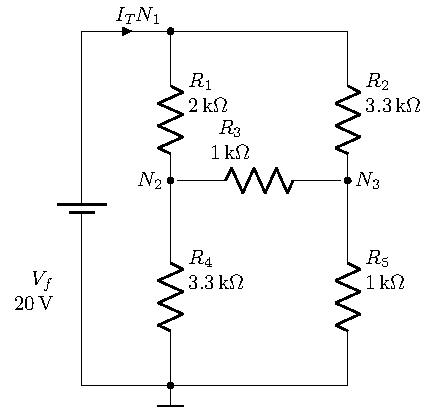
\includegraphics{figtemplate}
  \caption[Ejemplo de figura con tikz]{Ejemplo realizado con
    \texttt{tikz}.  Usted encuentra la plantilla en el directorio de
    figuras bajo el nombre \texttt{fig/figtemplate.tikz}.}
  \label{fig:figtemplate}
\end{figure}

\Lafigref{fig:figtemplate} muestra un ejemplo que se puede utilizar como
plantilla para generar figuras \texttt{tikz}.  La plantilla la
encuentra en el directorio de figuras y se llama
\code{figtemplate.tikz}.  En Internet se encuentran cientos de figuras
de ejemplo para realizar este tipo de figuras.

En el código fuente de la introducción \code{intro.tex} encuentra en
el diagrama de bloques otro ejemplo de cómo incrustar la figura Tikz
directamente en el lugar, aunque se advierte que eso no es
recomendable porque aumenta el tiempo de compilación del documento.
Considere esto particularmente si utiliza plataformas como
\href{https://overleaf.com}{Overleaf}, que tiene un tiempo de
compilación limitado.


\subsubsection{Figuras ltxfig/psfrag}

\index{psfrag}\index{ltxfig}
Cuando en el subdirectorio \texttt{fig/} se encuentran dos archivos con el
mismo nombre pero extensiones \texttt{ltxfig} y \texttt{psfrag}, por ejemplo
\texttt{prueba.ltxfig} y \texttt{prueba.psfrag}, entonces el Makefile asume que
usted desea crear una figura a partir del archivo \texttt{prueba.ltxfig},
creado con el programa \texttt{XFig}, sustituyendo los textos ahí presentes con
texto formateado con LaTeX.

\Lafigref{fig:ltxfig} ha sido creada con este esquema.  Revise los
archivos correspondientes en el directorio de figuras
\texttt{fig/ltxfig\_prototipo.*} para más detalles sobre su uso.

\begin{figure}[htb]
  \centering
  
\includegraphics[width=0.9\textwidth]{ltxfig_prototipo}
  \caption{Ejemplo de imagen ltxfig/psfrag}
  \label{fig:ltxfig}
\end{figure}

\subsubsection{Figuras pstricks}  

\index{pstricks} Los archivos con extensión \texttt{.pstricks} en el
directorio \texttt{fig} se utilizan para generar cualquier tipo de
imágenes según el código que se contenga.  Es un concepto más general
que el el utilizado con el \texttt{ltxfig} de la sección anterior.
\Lafigref{fig:pstricks} ha sido creada con este esquema.  Puede revisar
los archivos \texttt{prototipo\_gnuplot*} como un ejemplo de su uso,
en donde de un archivo gnuplot (\texttt{\_.gp}) se genera un archivo
\texttt{\_.eps}, el cual es incluido en el archivo \texttt{.pstricks}
sustituyendo cadenas de texto por código LaTeX.

\begin{figure}[htb]
  \centering
  
\includegraphics{prototipo_gnuplot}
  \caption{Ejemplo de imagen gnuplot/pstricks}
  \label{fig:pstricks}
\end{figure}

\subsubsection{Subfiguras}

En la plantilla ya se incluye el paquete \code{subcaption}, que es el
sucesor del paquete \code{subfig} que a su vez es el sucesor de
\code{subfigure}.  Los dos paquetes anteriores tienen muchos problemas
con el paquete \code{hyperref} y por tanto es mejor evitarlos.
\Lafigref{fig:subfiguras} muestra un ejemplo con dos figuras, donde por
ejemplo, \lafigref{fig:subfigura_a} es un circuito.  La
documentación del paquete \code{subcaption} presenta abundancia de
casos con y sin leyendas en las subfiguras y cómo referenciarlas
correctamente.

\begin{figure}[htb]
  \centering
  \subcaptionbox{\label{fig:subfigura_a}}%
    {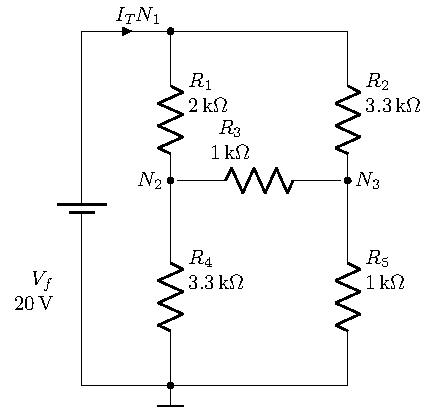
\includegraphics[scale=0.6]{figtemplate}}
  \subcaptionbox{\label{fig:subfigura_b}}%
    {
\includegraphics[scale=0.6]{prototipo_gnuplot}}
  \caption[Ejemplo de figuras con subcaption]{Este es un ejemplo de
      uso de subfiguras con subcaption.  (a) Un circuito.  (b) Una
      función.}
  \label{fig:subfiguras}
\end{figure}


\subsubsection{Entradas en el índice de figuras}

El índice de figuras debe servir para encontrar rápidamente dónde se
encuentra cierta figura.  El pie de la figura, indicado en \LaTeX con
\verb+\caption+ puede ser extenso, en especial para indicar detalles
de las figura.  Lo indicado con \verb+\caption+ es la entrada que por
defecto aparecerá en el índice de figuras.  Sin embargo, en el índice
la referencia a cada figura no debe superar la extensión de una línea
y debe únicamente dar la idea del contenido de la figura, para que
pueda ser encontrada rápidamente.  Para lograr esto en \LaTeX{} se
agrega un parámetro opcional con el texto del índice, de la siguiente
forma:
\begin{verbatim}
  \caption[Texto en el índice]{Texto al pie de la figura}
\end{verbatim}
Esto funciona también con \lastablas.


\subsection{Cuadros o tablas}

¿Se dice tabla o cuadro? Esta es una pregunta no tan simple de
responder.  \LaTeX, o mejor dicho el paquete \code{babel} para
español, por defecto define a las leyendas (\verb+\caption+) del
entorno \verb+table+ como \emph{cuadro}.  Sin embargo, en
Latinoamérica, en particular por influencia del inglés, se ha
extendido la traducción de \emph{table} como \emph{tabla}.

Formalmente en español se debería diferenciar entre ambas: la tabla
usualmente contiene datos que se referencian directamente, como las
tablas de logaritmos, la tabla periódica de los elementos, las tablas
de multiplicar, las tablas de transformadas, etc.  Los resultados de
un análisis experimental se sintetizan en lo que en español se
denomina \emph{cuadros}, y puesto que la mayoría de tesis e informes
de proyecto lo que se usan son precisamente \emph{cuadros}, entonces
\LaTeX\ para español define por defecto ese término.

En esta plantilla está activo el uso de \emph{tabla}, por ser esta la
tradición en la Escuela de Ingeniería Electrónica, pero basta eliminar
la opción \verb+es-tabla+ en el paquete \verb+babel+ en
\code{macros.tex} para reactivar el uso por defecto de \emph{cuadro}.

Si usted no tiene aún claro si desea usar \emph{cuadro} o
\emph{tabla}, utilice los comandos listados en
\latabref{tab:comandostab}, y así todo cambiará automáticamente de
acuerdo a la opción que se especifique para babel.  La tercera columna
muestra la salida de los comandos en la actual compilación del
documento.  Usted puede cambiar la opción de \verb+babel+ en
\code{macros.tex} y observar el cambio.

%\afterpage{% Esto es para forzar que la tabla salga después de la
%           % figura grande
\begin{table}[htb]
  \centering
  \caption[Comandos para cuadro o tabla]{Comandos definidos para
    cambiar cuadro o tabla según se indique al paquete babel.}
  \label{tab:comandostab}
  \begin{tabular}{llll}
    \toprule
    Comando & Con \verb+es-tabla+ & Sin \verb+es-tabla+ & Actualmente \\
    \midrule
    \verb+\cuadro+     & tabla      & cuadro      & \cuadro \\  
    \verb+\Cuadro+     & Tabla      & Cuadro      & \Cuadro \\  
    \verb+\elcuadro+   & la tabla   & el cuadro   & \elcuadro \\  
    \verb+\Elcuadro+   & La tabla   & El cuadro   & \Elcuadro \\  
    \verb+\loscuadros+ & las tablas & los cuadros & \loscuadros \\
    \verb+\Loscuadros+ & Las tablas & Los cuadros & \Loscuadros \\
    \verb+\tabla+      & tabla      & cuadro      & \tabla \\  
    \verb+\Tabla+      & Tabla      & Cuadro      & \Tabla \\  
    \verb+\latabla+    & la tabla   & el cuadro   & \latabla \\  
    \verb+\Latabla+    & La tabla   & El cuadro   & \Latabla \\  
    \verb+\lastablas+  & las tablas & los cuadros & \lastablas \\
    \verb+\Lastablas+  & Las tablas & Los cuadros & \Lastablas \\   
    \verb+\tabref{label}+
                       & tabla\verb+~\ref{label}+
                       & cuadro\verb+~\ref{label}+
                       & \tabref{tab:comandostab} \\
    \verb+\Tabref{label}+
                       & Tabla\verb+~\ref{label}+
                       & Cuadro\verb+~\ref{label}+
                       & \Tabref{tab:comandostab} \\
    \verb+\latabref{label}+
                       & la tabla\verb+~\ref{label}+
                       & el cuadro\verb+~\ref{label}+
                       & \latabref{tab:comandostab} \\
    \verb+\Latabref{label}+
                       & La tabla\verb+~\ref{label}+
                       & El cuadro\verb+~\ref{label}+
                       & \Latabref{tab:comandostab} \\
    \bottomrule
  \end{tabular}
\end{table}
%}

Observe que el comando \verb+\tabref+ se encarga de que la palabra
\emph{\tabla} quede como parte del enlace, mientras que si usted usa
directamente \verb+\ref+ entonces únicamente el número quedará
enlazado.

\subsubsection{Figuras enormes de una página en horizontal}

En ocasiones, es necesario colocar una figura o \tabla\ grande que no
cabe en el formato vertical de página.  Para esto, el entorno
\verb+sidewaysfigure+ permite rotar el contenido, aunque esto deja la
página en el archivo PDF generado en posición vertical, de modo que
cuando se lea por medios electrónicos, será incómodo interpretarlo, a
menos que activamente se rote todo el documento.  Una mejor opción es
entonces indicar directamente en el archivo PDF que se presente una
página en particular de forma horizontal, como lo ilustra la
\figref{fig:large}.
\afterpage{%
\clearpage
\begin{rotatepage}
\begin{sidewaysfigure}
  \centering
  
\includegraphics[width=\textheight]{ltxfig_prototipo}
  \caption{Ejemplo de figura enorme.}
  \label{fig:large}
\end{sidewaysfigure}
\end{rotatepage}
}
\clearpage %% Necesario aquí porque el verbatim que sigue confunde a latex



Para eso se ha definido en la plantilla un entorno sencillo denominado
\verb+rotatepage+.  Se usa de la siguiente forma:
%
\begin{verbatim}
\afterpage{%
  \clearpage
  \begin{rotatepage}
    \begin{sidewaysfigure}
      \centering
      
\includegraphics[width=\textheight]{ltxfig_prototipo}
      \caption{Ejemplo de figura enorme.}
    \end{sidewaysfigure}
  \end{rotatepage}
}
\end{verbatim}
%
El comando \verb+\afterpage+ da la instrucción de ejecutar el código
indicado justo después de terminar la página actual, en donde se
ordena primero pasar la página y sacar todos los objetos flotantes que
hayan quedado pendientes.  Esto tendrá el efecto secundarios de que si
en el resto de la página donde se coloca la inclusión de la figura hay
otros objetos flotantes, estos se colocarían primero.
%
Por ello, puede ser necesario que usted tenga que manipular esos
objetos flotantes para que aparezcan en otros lugares.

Siguiendo con el código de ejemplo, el entorno \verb+rotatepage+
intenta colocar los comandos de PDF necesarios para rotar la página.
Su implementación es muy sencilla y puede fallar.  Puede revisar su
implementación en el archivo {macros.tex}.



\subsection{Código}

Si usted necesita poner un ejemplo de código de descripción de
hardware o de algún lenguaje de programación, evite usar
``pantallazos'' pues al ser imágenes raster tiene baja calidad.

Puede insertar al código como figuras.  Si por la naturaleza del tema
de su proyecto o tesis hay más de diez ejemplos de código, quizá deba
buscar cómo agregar un nuevo tipo de objetos flotantes.

Se recomienda el uso del paquete \verb+listings+.  La plantilla define
en el archivo \code{macros.tex} un entorno para verilog, como se ilustra en la \figref{fig:verilog}.

\begin{figure}[htb]
  \begin{lstlisting}[style={verilog-style}]
    //-----------------------------------------------------
    // Design Name : mux_using_case
    // File Name   : mux_using_case.sv
    // Function    : 2:1 Mux using Case
    //-----------------------------------------------------
    module  mux_using_case(
      input  wire  din_0         , // Mux first input
      input  wire  din_1         , // Mux Second input
      input  wire  sel           , // Select input
      output reg [1:0]  mux_out    // Mux output (BUG IN HERE)
    );
    //-------------Code Starts Here---------
    always @ (*)
    MUX : begin
      case (sel) 
        1'b0 : mux_out = din_0;
        1'b1 : mux_out = din_1;
      endcase 
    end 
    
    endmodule //End Of Module mux
  \end{lstlisting}
  \caption[Ejemplo de código con listings.]{Ejemplo de uso de \code{listings}
    para insertar código Verilog, pero puede usarse para otros
    lenguajes.}
  \label{fig:verilog}
\end{figure}

\subsection{Referencias bibliográficas}

\index{referencias}\index{BibTeX} Todo concepto o idea tomado de otros
autores contar con la respectiva referencia. En redacción técnica de
ingeniería rara vez se utiliza la cita textual, así que es necesario
reformular las ideas y conceptos con palabras propias. En ingeniería
electrónica se utilizan los formatos de referencia de la IEEE o la
ACM, que son numéricos, encerrados entre paréntesis cuadrados (por
ejemplo, ``En \cite{Davis1963} se propuso un nuevo algoritmo'', o ``En
\cite{ProakisManolakis1998} los autores proponen tomar las ventajas de
los algorimos presentados
en~\cite{Oppenheim1998,Roberts2005,Haykin2001} por medio del método de
Newton \cite{Burrus1998} conocido en el área de optimización
lineal.''). La referencia es parte de las frases, así que si la frase
termina con la referencia para indicar la idea, ésta debe estar antes
del punto final o demás signos de puntuación: ``La capacidad de
memoria también sigue una Ley similar a la de Moore \cite{Octave}. Los
siguientes son los aspectos a tomar en cuenta en el diseño del sistema
\cite{Lindner2002}:''.  Las referencias múltiples usan un solo comando
\verb|\cite{Sorial2003,Shilov1973}|~\cite{Soria2003,Shilov1973}.

Se recomienda utilizar BibLaTeX para indicar las referencias
bibliográficas.  Actualmente herramientas como Mendeley, Zotero u
otras similares simplifican la administración de las referencias y
pueden exportar al formato BibTeX.

Si usa estos formatos, recuerde en los autores con dos apellidos
siempre usar
\begin{center}
  \code{author=\{apellidos, nombres and apellidos, nombres\}}  
\end{center}
o de lo contrario la generación de las referencias será incorrecta.

\subsection{Extensión}

\index{extensión}
Una tesis de licenciatura no debe sobrepasar las 120 páginas incluyendo
apéndices y los formalismos desde portada hasta índices.

El cuerpo de la tesis (desde introducción hasta conclusiones) usualmente se
extiende desde 45 páginas hasta no más de 80, dependiendo de la problemática
tratada.

No es necesario reproducir contenidos de otras fuentes: agregue las referencias
a dichas fuentes, y limítese a enunciar lo estrictamente necesario para
comprender sus propuestas de solución.

Contenidos que se salen de la línea principal de la tesis se colocan
en apédices, a los que se hace breve referencia (ver
apéndice~\ref{apx:apendice}).

\section{Sobre esta plantilla \LaTeX}

Esta plantilla \LaTeX pretende simplificar varios pasos en la creación
del documento de tesis.  Toda la configuración, incluyendo su nombre,
su número de carné, el nombre abreviado, el título del documento, la
fecha de defensa, el nombre de su asesor y sus lectores, etc.\ se
especifica en el archivo \code{config.tex}.

\subsection{Marcar asuntos pendientes}

La plantilla tiene dos ``\emph{modos}'' de operación: normal y
borrador (\emph{draft}).  En el archivo \texttt{config.tex}, en las
líneas 12 y 13 usted encuentra el código

\begin{verbatim}
\setboolean{draftmode}{true}            % turn draft mode on
%\setboolean{draftmode}{false}          % turn draft mode off
\end{verbatim}

Con el modo borrador, se activan ciertos comandos y funcionalidades
útiles en el proceso de elaboración de la tesis, pero que deben ser
desactivados al final, antes de entregar la tesis.  Por ejemplo, se
activa el pie de página que dice ``\emph{Borrador: fecha}'', y se
activa el índice titulado ``Revisar''.  En dicho índice aparecen las
páginas en donde se hayan utilizado alguno de los siguientes comandos:
\begin{compactitem}
\item \verb+\boxcomment{comentario}+ Crea una caja en el margen de página con
  el comentario indicado.
\item \verb+\explain{comentario}+ Crea una caja en el margen de página con
  el comentario indicado, con una flecha hacia la derecha para indicar qué en
  concreto debe ser revisado.
\item \verb+\chk{comentario}+ Crea una caja en el margen con símbolo de
  ``chequeado'' y el comentario indicado.
\item \verb+\TODO{comentario}+ Crea una caja grande de fondo sombreado con el
  comentario indicado.
\end{compactitem}

En este párrafo se\chk{resultado de chk} utilizan algunos de estos comandos
para ilustrar su efecto.  El \verb+\chk+ como puede observar tiene sentido
usarlo para marcar que algo está casi listo.  Por otro lado \explain{explain}
el comando \verb+\explain+ permite marcar algo que requiere ser revisado en
redacción, valores, etc.  El \verb+\boxcomment+\boxcomment{La caja simple}
solo pone una marca al margen.

\TODO{Finalmente el comando \texttt{TODO} coloca esta caja gris.}

Si usted desativa el modo draft, desaparecen todas las marcas
anteriores, y desaparece el índice ``Revisar''.  En éste índice
aparecen todas las páginas en donde se utilizaron estos comandos con
los respectivos comentarios, lo que permite encontrar rápidamente
detalles que usted indicó que debe revisar.

\subsection{Índices}

Como índice se conoce la lista de términos claves con su respectiva
página.  Usualmente aparece al final del documento.  La plantilla
ofrece varios comandos para simplificar el uso estandar del comando de
\LaTeX\ \verb+\index{término}+ que coloca al término indicado en el
índice.  Con \verb+\nt[indice]{término}+ (\emph{new term}) usted
indica la entrada principal del término, que aparece en el texto en el
índice, es decir, en el índice aparece lo que indique en vez de
``indice'' y en el texto aparece lo que indique ``término'';
\verb+\ot{término}+ agrega una entrada secundaria al término.
